\chapter{Results}
\label{chap:5}
%
TODO


We plot the mean and the standard deviation for all kernel runs. One run consists a number of trails-cf averaged  Due to high jitter on the average of each kernel run, all plots are smoothed by a moving mean of five. Also, the standard deviation values are divided by five to maintain readability when three or four different kernel graphs are present in one plot.

\begin{figure}[h]
\centering
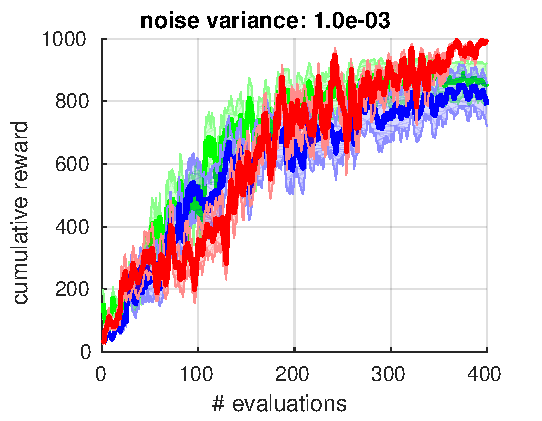
\includegraphics[width=.245\textwidth]{/home/sebastian/Documents/bscThesis/img/noisecompare/1.pdf}
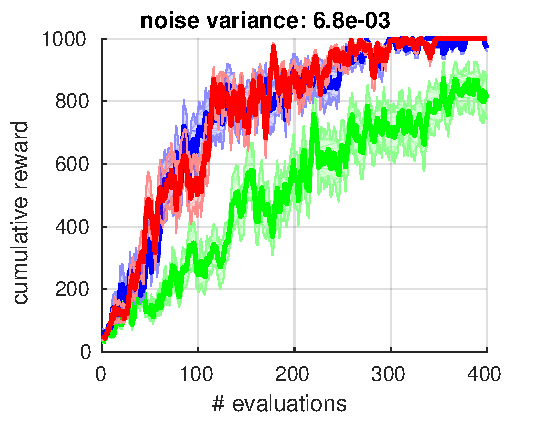
\includegraphics[width=.245\textwidth]{/home/sebastian/Documents/bscThesis/img/noisecompare/2.pdf}
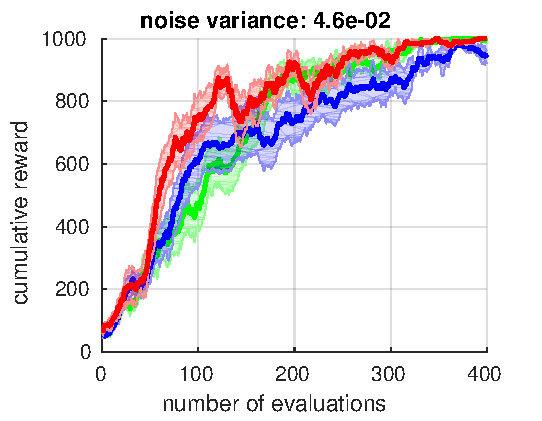
\includegraphics[width=.245\textwidth]{/home/sebastian/Documents/bscThesis/img/noisecompare/3.pdf}
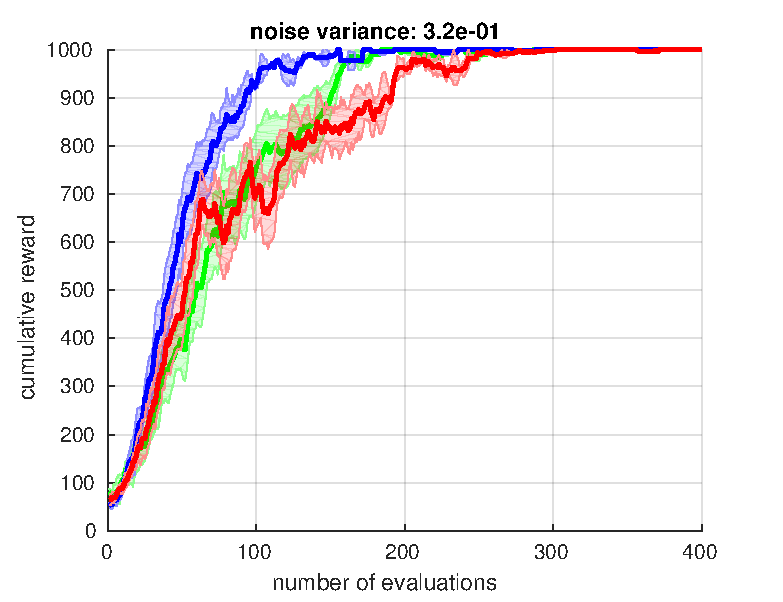
\includegraphics[width=.245\textwidth]{/home/sebastian/Documents/bscThesis/img/noisecompare/4.pdf}

\medskip

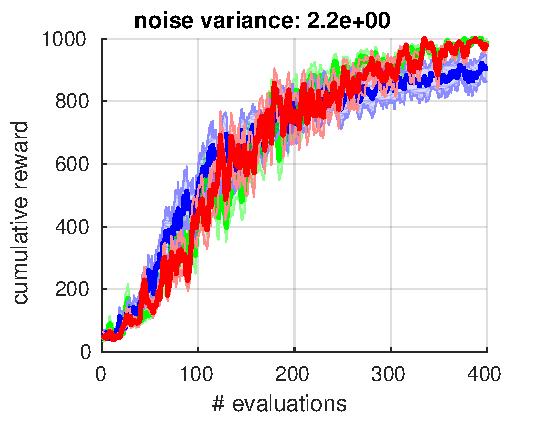
\includegraphics[width=.245\textwidth]{/home/sebastian/Documents/bscThesis/img/noisecompare/5.pdf}
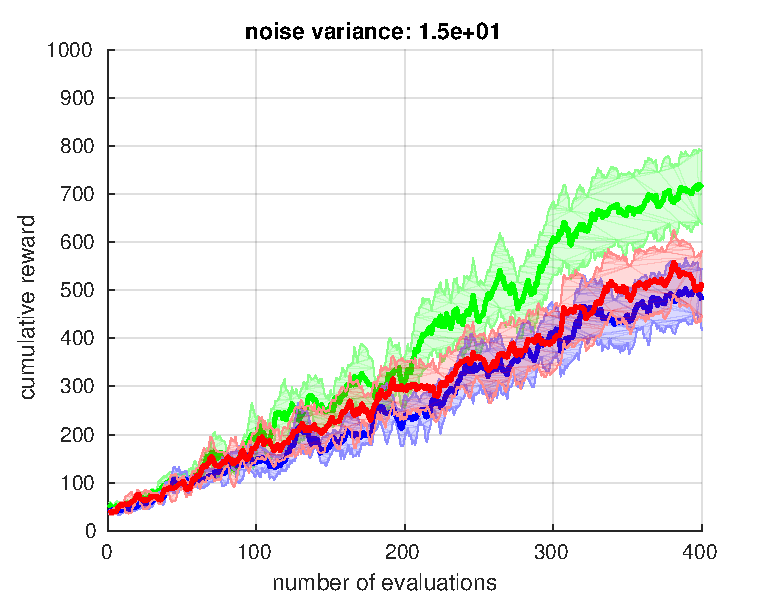
\includegraphics[width=.245\textwidth]{/home/sebastian/Documents/bscThesis/img/noisecompare/6.pdf}
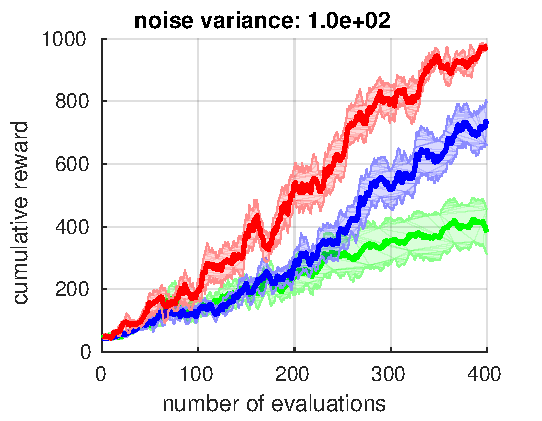
\includegraphics[width=.245\textwidth]{/home/sebastian/Documents/bscThesis/img/noisecompare/7.pdf}
\raisebox{\height}{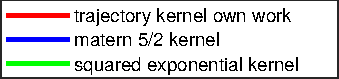
\includegraphics[width=.245\textwidth]{/home/sebastian/Documents/bscThesis/img/noisecompare/legend.pdf}}

\caption{Noise level comparison on the Matlab Cart Pole implementation with the local Bayesian optimizer. The noise levels are logarithmically spaced and sorted in ascending order from $10^{-3}$ to $10^2$. Each kernel graph contains the average over 5 trials.}
\label{pics:blablabla}
\end{figure}
